\documentclass[tikz,border=12pt]{standalone}
\usepackage[T1]{fontenc}
\usepackage{mathpazo}
\usepackage{amsmath,amssymb}
\usetikzlibrary{arrows.meta, calc, patterns, decorations.pathreplacing}

\definecolor{stblue}{HTML}{7B97AD}
\definecolor{rwgold}{HTML}{B8995E}
\definecolor{sage}{HTML}{7A9A7E}
\definecolor{dkbrown}{HTML}{3D3530}
\definecolor{wmgray}{HTML}{7B7067}
\definecolor{cream}{HTML}{F9F6F0}
\definecolor{border}{HTML}{D4C9B8}
\definecolor{terracotta}{HTML}{C47A6A}
\definecolor{lavender}{HTML}{907EA0}
\definecolor{rosewood}{HTML}{AD8480}

\begin{document}
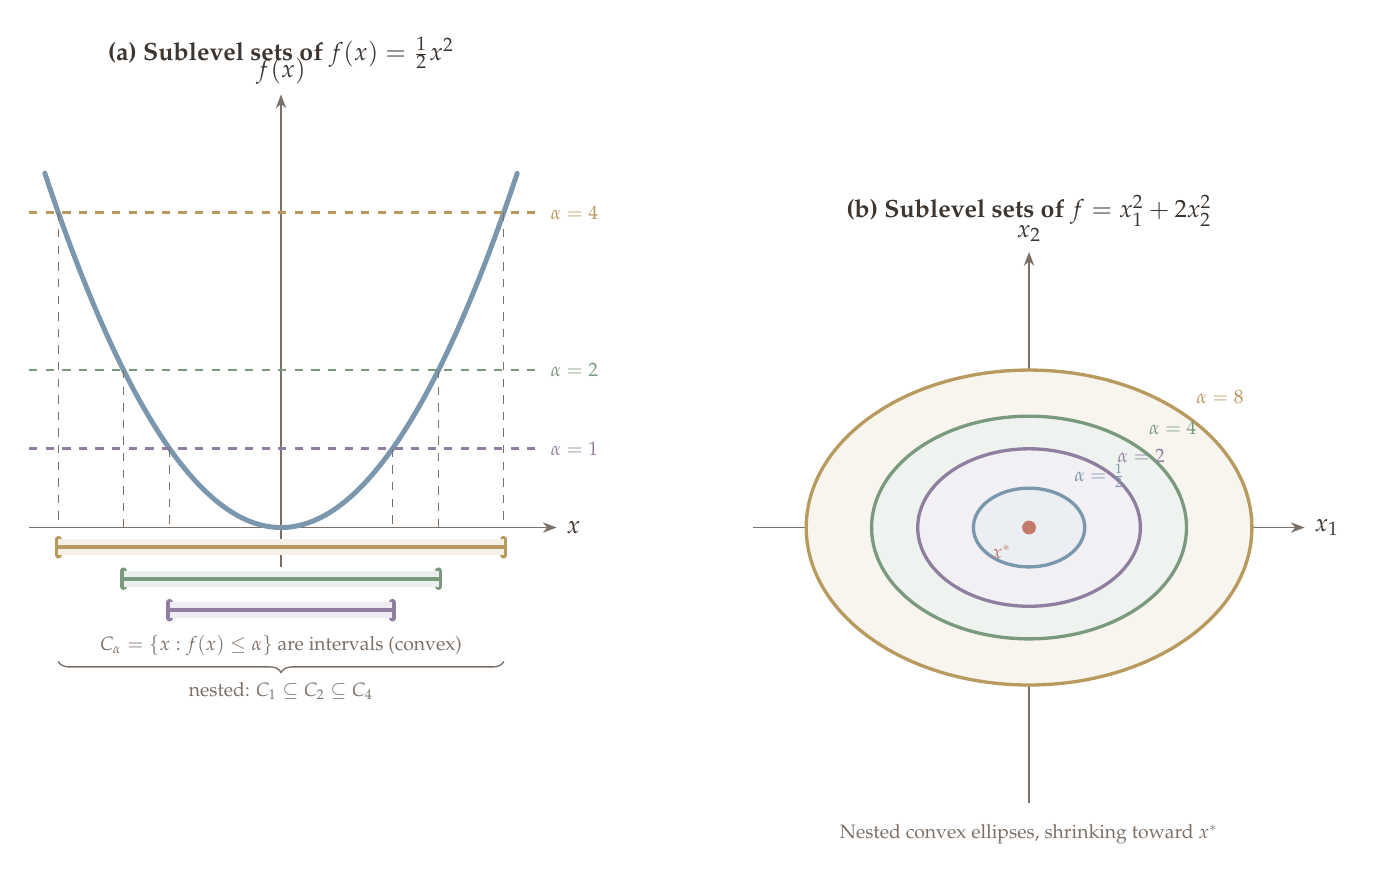
\begin{tikzpicture}[
  axis/.style={-{Stealth[length=5pt]}, wmgray, line width=0.6pt},
  curve/.style={line width=1.8pt, line cap=round},
  label/.style={dkbrown, font=\small},
]

% ===== Left panel: 1D sublevel sets =====
\begin{scope}[shift={(0,0)}]
  \draw[axis] (-3.2,0) -- (3.5,0) node[right, label] {$x$};
  \draw[axis] (0,-0.5) -- (0,5.5) node[above, label] {$f(x)$};

  % Convex curve: x^2/2
  \draw[curve, stblue, domain=-3:3, samples=80, smooth]
    plot (\x, {0.5*\x*\x});

  % Alpha = 4 level
  \draw[rwgold, line width=1pt, dashed] (-3.2, 4) -- (3.3, 4);
  \node[rwgold, font=\scriptsize, anchor=west] at (3.3, 4) {$\alpha = 4$};
  % Sublevel bracket
  \draw[rwgold, line width=2.5pt, line cap=round] (-2.83, -0.15) -- (-2.83, -0.35);
  \draw[rwgold, line width=2.5pt, line cap=round] (2.83, -0.15) -- (2.83, -0.35);
  \fill[rwgold!15] (-2.83, -0.15) rectangle (2.83, -0.35);
  \draw[rwgold, line width=1.5pt] (-2.83, -0.25) -- (2.83, -0.25);

  % Alpha = 2 level
  \draw[sage, line width=1pt, dashed] (-3.2, 2) -- (3.3, 2);
  \node[sage, font=\scriptsize, anchor=west] at (3.3, 2) {$\alpha = 2$};
  % Sublevel bracket
  \draw[sage, line width=2.5pt, line cap=round] (-2, -0.55) -- (-2, -0.75);
  \draw[sage, line width=2.5pt, line cap=round] (2, -0.55) -- (2, -0.75);
  \fill[sage!15] (-2, -0.55) rectangle (2, -0.75);
  \draw[sage, line width=1.5pt] (-2, -0.65) -- (2, -0.65);

  % Alpha = 1 level
  \draw[lavender, line width=1pt, dashed] (-3.2, 1) -- (3.3, 1);
  \node[lavender, font=\scriptsize, anchor=west] at (3.3, 1) {$\alpha = 1$};
  % Sublevel bracket
  \draw[lavender, line width=2.5pt, line cap=round] (-1.414, -0.95) -- (-1.414, -1.15);
  \draw[lavender, line width=2.5pt, line cap=round] (1.414, -0.95) -- (1.414, -1.15);
  \fill[lavender!15] (-1.414, -0.95) rectangle (1.414, -1.15);
  \draw[lavender, line width=1.5pt] (-1.414, -1.05) -- (1.414, -1.05);

  % Vertical dashed drop lines
  \draw[wmgray, line width=0.4pt, dashed] (-2.83, 4) -- (-2.83, 0);
  \draw[wmgray, line width=0.4pt, dashed] (2.83, 4) -- (2.83, 0);
  \draw[wmgray, line width=0.4pt, dashed] (-2, 2) -- (-2, 0);
  \draw[wmgray, line width=0.4pt, dashed] (2, 2) -- (2, 0);
  \draw[wmgray, line width=0.4pt, dashed] (-1.414, 1) -- (-1.414, 0);
  \draw[wmgray, line width=0.4pt, dashed] (1.414, 1) -- (1.414, 0);

  % Labels
  \node[dkbrown, font=\small\bfseries, anchor=south] at (0, 5.7) {(a) Sublevel sets of $f(x) = \tfrac{1}{2}x^2$};
  \node[wmgray, font=\scriptsize] at (0, -1.5) {$C_\alpha = \{x : f(x) \leq \alpha\}$ are intervals (convex)};

  % Nested annotation
  \draw[decorate, decoration={brace, amplitude=4pt, mirror}, wmgray, line width=0.5pt]
    (-2.83, -1.7) -- (2.83, -1.7) node[midway, below=4pt, wmgray, font=\scriptsize] {nested: $C_1 \subseteq C_2 \subseteq C_4$};
\end{scope}

% ===== Right panel: 2D sublevel sets (ellipses) =====
\begin{scope}[shift={(9.5,0)}]
  \draw[axis] (-3.5,0) -- (3.5,0) node[right, label] {$x_1$};
  \draw[axis] (0,-3.5) -- (0,3.5) node[above, label] {$x_2$};

  % f(x1,x2) = x1^2 + 2*x2^2
  % C_alpha: x1^2 + 2*x2^2 <= alpha
  % => x1^2/alpha + x2^2/(alpha/2) <= 1
  % semi-axes: sqrt(alpha) along x1, sqrt(alpha/2) along x2

  % Alpha = 8 (outermost): semi-axes 2.83, 2
  \fill[rwgold!10] (0,0) ellipse (2.83 and 2);
  \draw[rwgold, line width=1.2pt] (0,0) ellipse (2.83 and 2);
  \node[rwgold, font=\scriptsize, anchor=south west] at (2.0, 1.45) {$\alpha = 8$};

  % Alpha = 4: semi-axes 2, 1.414
  \fill[sage!12] (0,0) ellipse (2 and 1.414);
  \draw[sage, line width=1.2pt] (0,0) ellipse (2 and 1.414);
  \node[sage, font=\scriptsize, anchor=south west] at (1.4, 1.05) {$\alpha = 4$};

  % Alpha = 2: semi-axes 1.414, 1
  \fill[lavender!12] (0,0) ellipse (1.414 and 1);
  \draw[lavender, line width=1.2pt] (0,0) ellipse (1.414 and 1);
  \node[lavender, font=\scriptsize, anchor=south west] at (1.0, 0.7) {$\alpha = 2$};

  % Alpha = 0.5 (innermost): semi-axes 0.707, 0.5
  \fill[stblue!15] (0,0) ellipse (0.707 and 0.5);
  \draw[stblue, line width=1.2pt] (0,0) ellipse (0.707 and 0.5);
  \node[stblue, font=\scriptsize, anchor=south west] at (0.45, 0.38) {$\alpha = \tfrac{1}{2}$};

  % Minimum
  \fill[terracotta] (0,0) circle (2.5pt);
  \node[terracotta, font=\scriptsize, anchor=north east] at (-0.1, -0.1) {$x^*$};

  \node[dkbrown, font=\small\bfseries, anchor=south] at (0, 3.7) {(b) Sublevel sets of $f = x_1^2 + 2x_2^2$};
  \node[wmgray, font=\scriptsize] at (0, -3.9) {Nested convex ellipses, shrinking toward $x^*$};
\end{scope}

\end{tikzpicture}
\end{document}
